\documentclass{beamer}
\DeclareFontShape{OT1}{cmss}{b}{n}{<->ssub * cmss/bx/n}{} 
\usetheme{Szeged}
\usecolortheme{beaver}
\usepackage{amsmath}
\usepackage{amsfonts}
\usepackage{mathbbol}
\usepackage{xcolor} % before tikz or tkz-euclide if necessary
\usepackage{tkz-euclide} % no need to load TikZ
\usepackage{multirow}
\usepackage{lmodern}
\usepackage{bm}
\usepackage{subcaption}
%\usepackage{subfigure}

\usepackage[
backend=biber,
style=authoryear-icomp,
sortlocale=de_DE,
natbib=true,
url=false, 
doi=true,
eprint=false
]{biblatex}
\addbibresource{../Bibliography/main_ML.bib}



\titlegraphic{
\includegraphics[width=2cm]{../Figures/UAMS_RGB.png}
}


\title{Neuroinformatics Journal Club\\ Dynamic Brain Networks (HMM) \\ Electrophysiology}
\author{Horacio G\'omez-Acevedo\\ Department of Biomedical Informatics\\
	University of Arkansas for Medical Sciences}

\begin{document}
	\begin{frame}[plain]
		\maketitle
	\end{frame}
	
	\begin{frame}{Today's paper}
		\begin{figure}[h]
			\centering
			%	\begin{subfigure}{0.4\textwidth}
				%		\centering
				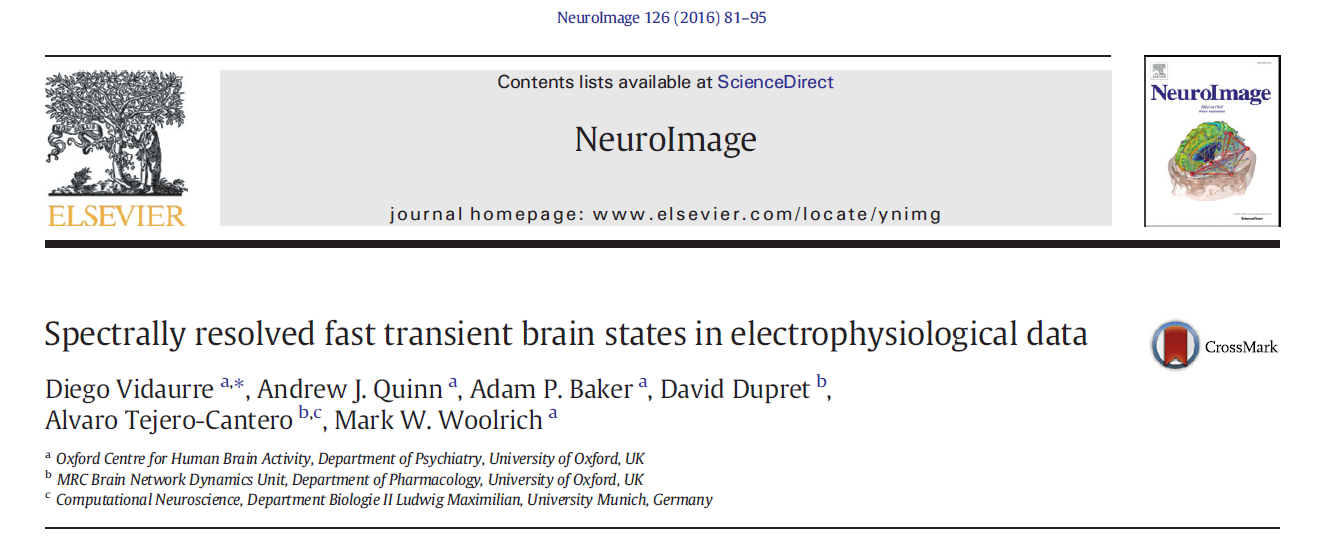
\includegraphics[scale=0.45]{../Figures/vidaurre_paper2.png}
				%	\end{subfigure}
		\end{figure}
	\end{frame}
	
	
%	\begin{frame}{Hidden Markov Models}
%		The implementation of Hidden Markov models dates back in the late 60's by Leonard Baum and collaborators. It is still an active area of research. 	
%		
%		What is a Markov chain?
%		\begin{figure}[h]
%			\centering
%			%	\begin{subfigure}{0.4\textwidth}
%				%		\centering
%				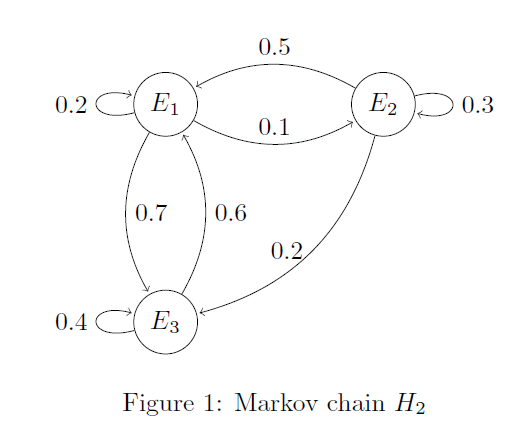
\includegraphics[scale=0.6]{../Figures/fig_markov_chain.png}
%				%	\end{subfigure}
%		\end{figure}
%		
%		
%	\end{frame}
%	
%	\begin{frame}{Hidden Markov Chains}
%		The fair casino problem 
%		\begin{itemize}
%			\item You don't know if the dealer has a fair or unfair coin (Hidden states)
%			\item You only observe the output (Emissions)
%		\end{itemize}
%		\begin{figure}[h]
%			\centering
%			%	\begin{subfigure}{0.4\textwidth}
%				%		\centering
%				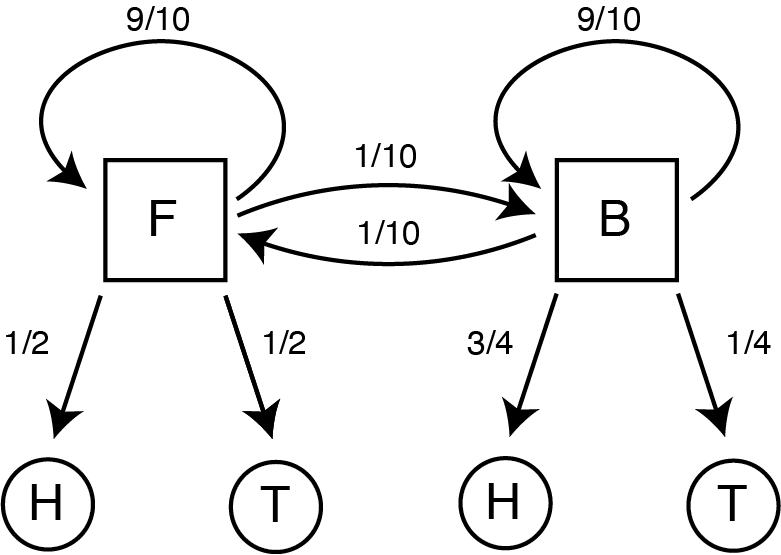
\includegraphics[scale=0.6]{../Figures/hmm_fair_casino.png}
%				%	\end{subfigure}
%		\end{figure}
%	\end{frame}
%	
	\begin{frame}{Workflow}
	
		
		\begin{figure}[h]
			\centering
			%	\begin{subfigure}{0.4\textwidth}
				%		\centering
				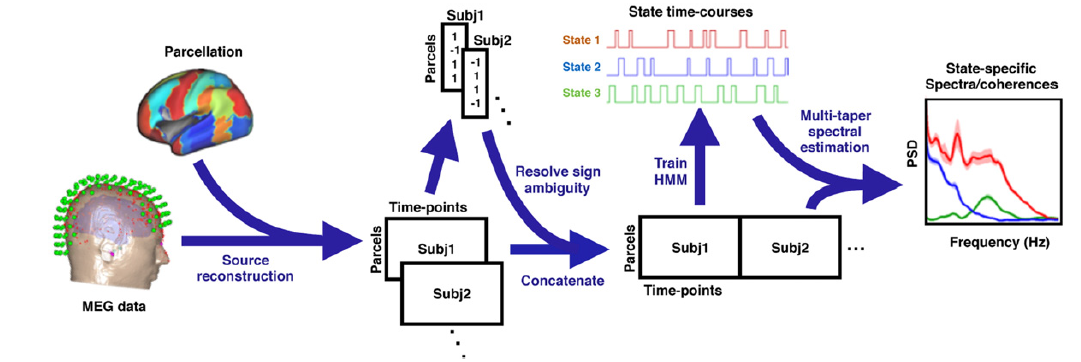
\includegraphics[scale=0.5]{../Figures/fig_vidaurre2_1.png}
				%	\end{subfigure}
		\end{figure}
	\end{frame}
\begin{frame}{Modeling ingredients}
	The paper follows some of the similar themes as the previous one
	\begin{itemize}
		\item Hidden Markov Models
		\item Autoregressive models
	\end{itemize}
To make things "interesting" it adds some more topics
\begin{itemize}
	\item Bayesian methods
	\item Some Fourier Analysis
\end{itemize}

\end{frame}

\begin{frame}{Basic Setup}
	We consider $K$ hidden states, and $T$ time points.
	
	Let $\mathbf{y}_t^N$ be the multichannel source signal. 
	
	The construction of the multivariate autoregressive (MAR) model is different than before. 
	\begin{equation}
		\mathbf{y}'_t | x_t =k  \sim {\cal N}\left(\sum_{l\in A} 
		\mathbf{y}'_{t-1} \mathbf{W}_l^{(k)}, \Sigma^{(k)}\right)
	\end{equation}
Don't panic (just yet)
\begin{itemize}
\item $\mathbf{y}'_t | x_t =k $ This part refers to as the emission at time $t$ when you are in the hidden state $k$. It is the transpose of the vector of $N$ entries.
\item The $\cal N$ refers to the multivariate normal distribution. In the 1-dimensional case ${\cal N}(\mu, \sigma)$ the $\mu$ is transformed into a vector, and the $\sigma$ by a matrix (variance-covariance). 

\end{itemize}
	
\end{frame}
\begin{frame}{Basic Setup (cont)}
\begin{itemize}
	\item $\mathbf{y}'_{t-1} \mathbf{W}_l^{(k)}$ refers to as the MAR component. The matrix $ \mathbf{W}_l^{(k)}$ is of type $N\times N$ for the $k$th (hidden) state for the lag $l$. We add all the individual contributions of each lag step.
	\item $\Sigma^{(k)}$ is the noise covariance matrix.   
\end{itemize}
The Markovian property 
\begin{equation}
	P(x_t=k_1|x_{t-1}=k_2)= \Theta_{k_1k_2}, \quad P(x_t=k)= \eta_k
\end{equation}
\end{frame}

	\begin{frame}{Viterbi's representation HMMs}
		\begin{figure}[h]
			\centering
			%	\begin{subfigure}{0.4\textwidth}
				%		\centering
				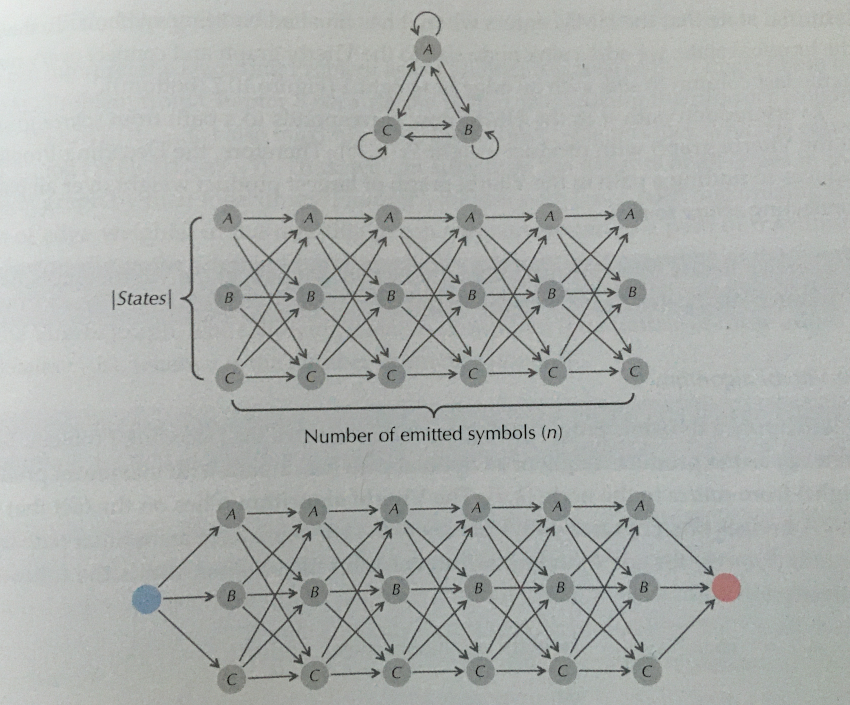
\includegraphics[scale=0.6]{../Figures/fig_hmm.png}
				%	\end{subfigure}
		\end{figure}
	\end{frame}

	\begin{frame}{MAR model}
	
	
	\begin{figure}[h]
		\centering
		%	\begin{subfigure}{0.4\textwidth}
			%		\centering
			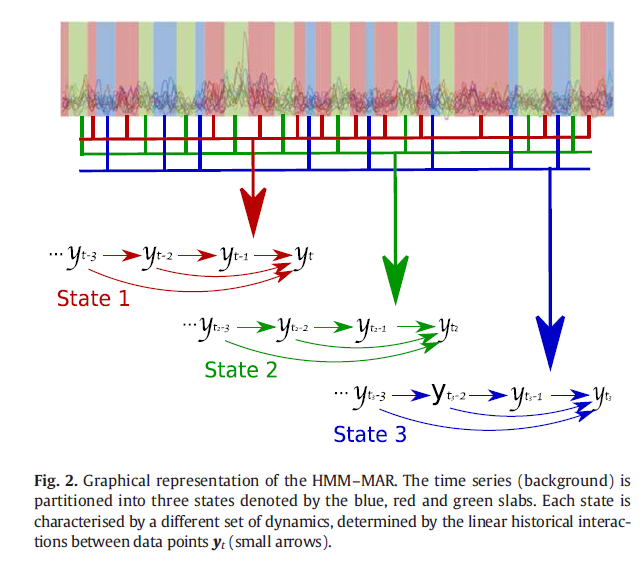
\includegraphics[scale=0.5]{../Figures/fig_vidaurre2_2.png}
			%	\end{subfigure}
	\end{figure}
\end{frame}
	
	\begin{frame}{MAR model (cont)}
	The paper key component for the MAR section is the $\cal A$ set.
	It contains the number of previous steps to be considered
	\begin{equation}
		{\cal A}= \{ P_0 +1,P_0+Q , P_0+ \left\lfloor\frac{1}{2}Q^2\right\rfloor,\ldots,P\}
	\end{equation}
It calls it exponential due to the Taylor representation of the exponential function
\begin{equation*}
	\exp(X)= 1 + X + \frac{1}{2!}X^2 + \frac{1}{3!}X^3 + \cdots
\end{equation*}
	\end{frame}

\begin{frame}{Oh Bayes where art thou?}
	Unlike the traditional (frequentist) inference, the Bayesian approach tries to determine conclusions about a parameter $\theta$ or unobserved data $\overline{y}$ as probability statements.  For example, given the observed data $y$,  Bayesian statements are based on the conditionals such as  $P(\overline{y}|y)$ for {\it new data} $\overline{y}$, or $P(\theta|y)$ for a parameter $\theta$. So following our Bayes theorem,

\begin{equation}
	{\color{blue}P(\theta| y)}=\frac{{\color{red} P(\theta)} {\color{green}P(y|\theta)}}{\color{purple}P(y)}
	\label{eq:bayes2}
\end{equation}
where $P(y)= \sum_{\theta} P(\theta) P(y|\theta)$ (or in the continuous case $P(y)= \int P(\theta) P(y|\theta) d\theta$). 

The expression  $\color{red} P(\theta)$ is called the {\bf prior}, whereas  $\color{blue} P(\theta|y)$  is called {\bf posterior}, and $\color{green}P(y|\theta)$ is called {\bf likelihood}, and $\color{purple}P(y)$ is called {\bf evidence}. 

\end{frame}	

\begin{frame}{Oh Bayes where art thou? (cont)}
		\begin{figure}[h]
		\centering
		%	\begin{subfigure}{0.4\textwidth}
			%		\centering
			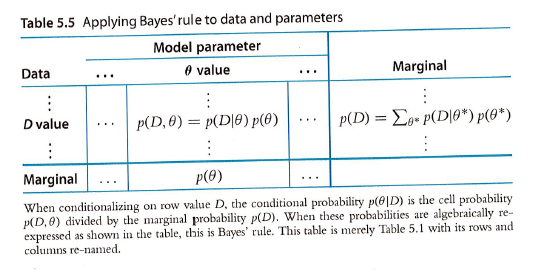
\includegraphics[scale=0.75]{../Figures/fig_bayes_table.png}
			%	\end{subfigure}
	\end{figure}
\end{frame}

\begin{frame}{Oh Bayes where art thou? (cont)}
	\begin{figure}[h]
		\centering
		%	\begin{subfigure}{0.4\textwidth}
			%		\centering
			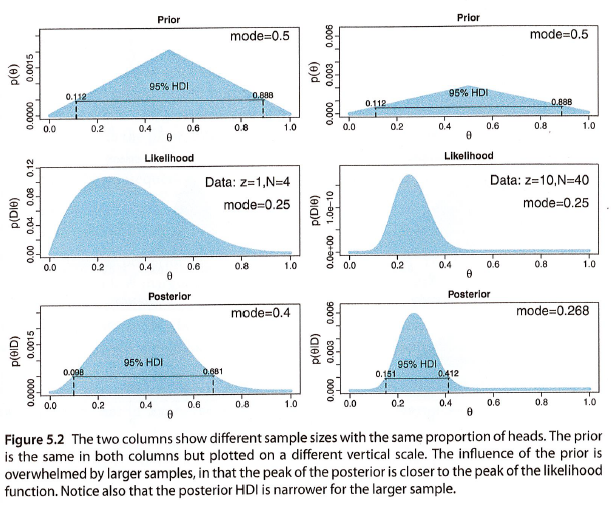
\includegraphics[scale=0.65]{../Figures/fig_bayes_prior.png}
			%	\end{subfigure}
	\end{figure}
\end{frame}


\begin{frame}{Oh Bayes where art thou?}
	The precision matrix is modeled with a Wishart distribution
	\begin{equation}
		\Omega^{(k)} \sim {\cal W}(t_0,\mathbf{B}_0)
	\end{equation}
 An example: Sample covariance for idd multivariate normal. You can think about it as a multivariate version of the Gamma distribution.
 
 \textbf{Priors}.
 
 We expect each state to be characterized by a certain set of connections and certain frequency profile... $\sigma_{ij}^{(k)}$ weight the presence of a specific connection between nodes $(i,j)$ when in state $k$. The precision $\alpha_j^{(k)}$ adaptively weight to the presence of interaction at a certain lag $l$ for all nodes when in state $k$.
 
 
\end{frame}

\begin{frame}{Bayes cont}
	
The authors generate a \textit{Hierarchical Bayes Model}
	\begin{equation}
		W_{l_{ij}}^{(k)} \sim {\cal N}(0, \sigma_{ij}^{(k)} \alpha_j^{(k)} )
	\end{equation}
	where 
	\begin{equation}
		\sigma_{ij}^{(k)}\sim \Gamma (\phi_0, d_0)
	\end{equation}
	\begin{equation}
		\alpha_j^{(k)} \sim \Gamma (\xi_0, d_0)
	\end{equation}
\end{frame}

\begin{frame}{Bayes cont}
	\begin{equation}
		\Theta_k \sim Dir(\nu_0) \quad \eta \sim Dir (\psi_0)
	\end{equation}
The Dirichlet distribution is the conjugate prior for the parameters of the normal multinomial distribution. 


\end{frame}

\begin{frame}{Inference of Model Parameters}
	
	Bayesian models are difficult to perform since the Bayes' rule involves computing the evidence (nasty math problem).
	Thus, the models are restricted to ones with \textit{simple} likelihood functions with corresponding formulas for prior distributions (called \textit{conjugate priors}) that play nice with the likelihood function. Another alternative is to use what is called \textit{variational approximation}. 
	
\end{frame}

\begin{frame}{Spectral Properties}
	The authors use something called \textit{Fourier Transform} to investigate find out the multiregion spectral properties of the state time courses.
	
	In a nutshell this methodology takes a real function $f$ and it produces a continuous function of frequency. 
	So, the expression
	\begin{equation}
		S(f)= \frac{}{R}\sum_{r=1}^{R} \sum_{t=1}^{T} \delta_t^{(r)}y_t \exp(-2\pi i f t)  
	\end{equation}


\end{frame}

%\begin{frame}{Fourier Transform}
%	\begin{figure}[h]
%	\centering
%	%	\begin{subfigure}{0.4\textwidth}
%		%		\centering
%		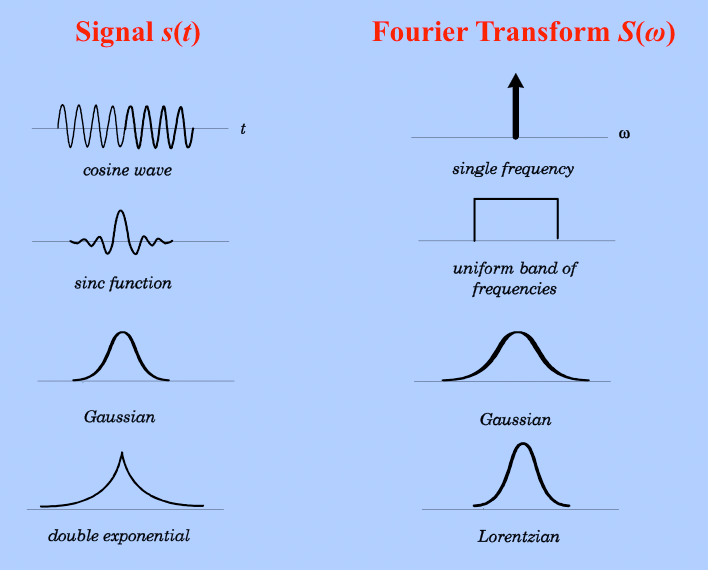
\includegraphics[scale=0.65]{../Figures/fig_fourier_transform.}
%		%	\end{subfigure}
%\end{figure}
%\end{frame}

	
	%\begin{frame}{References}
	%	Materials and some of the pictures are from \citep{calin}.
	%	\printbibliography 	
	
	%	I have used some of the graphs by hacking TiKz code from StakExchange, Inkscape for more aesthetic plots and other old tricks of \TeX
	
	%\end{frame}
	
	
\end{document}
